\chapter{Dispersion, Impedance, Reflection, and Transmission
 \label{chap:dispersion}}

%\setcounter{page}{1}

\renewcommand{\thefootnote}{\fnsymbol{footnote}}
\footnotetext[2]{Lecture notes by John Schneider.  {\tt
fdtd-dispersion.tex}}

\section{Introduction}

A dispersion relation gives the relationship between frequency and
the speed of propagation.  This relationship is rather simple in the
continuous world and is reviewed in the next section.  Unfortunately
dispersion in the FDTD is not as simple.  Nevertheless, it provides a
great deal of insight into the inherent limitations of the FDTD method
and hence it is important that one have at least a basic understanding
of it.

The tools developed in the analysis of FDTD dispersion can also be
used to determine the characteristic impedance of the grid.
Furthermore, as will be shown, knowing the dispersion relationship
one can obtain exact analytic expressions for the reflection and
transmission coefficients in the FDTD grid.

\section{Dispersion in the Continuous World}

Consider a plane wave propagating in the $+x$ direction in a
lossless medium.  In time-harmonic form the temporal and spatial
dependence of the wave are given by $\exp(j[\omega t-\beta x])$ where
$\omega$ is the frequency and $\beta$ is the phase constant (wave number).
The speed of the wave can be found by determining how fast a given
point on the wave travels.  In this context ``point'' is taken to mean
a point of constant phase.  The phase is dictated by $\omega t - \beta x$.
Setting this equal to a constant and differentiating with respect to
time gives
\begin{eqnarray}
  \frac{d}{dt}(\omega t-\beta x) &=& \frac{d}{dt}(\mbox{constant}), \\
  \omega - \beta \frac{dx}{dt} &=& 0. \label{eq:phase}
\end{eqnarray}
In this expression $x$ is taken to be the position which provides a
particular phase.  In that sense it is not an independent variable.
The location $x$ which yields the desired phase will change as a
function of time.  Therefore, $dx/dt$ is the speed of the wave, or,
more properly, the phase speed $c_p$.  Solving \refeq{eq:phase} for the
phase speed yields
\begin{equation}
  c_p = \frac{dx}{dt} = \frac{\omega}{\beta}.
\end{equation}
This is apparently a function of frequency, but for a plane wave the
phase constant $\beta$ is given by $\omega\sqrt{\mu\epsilon}$.  Thus
the phase speed is
\begin{equation}
  c_p = \frac{\omega}{\omega\sqrt{\mu\epsilon}} 
  = \frac{1}{\sqrt{\mu_r\mu_0\epsilon_r\epsilon_0}} 
  = \frac{c}{\sqrt{\mu_r\epsilon_r}}
\end{equation}
where $c$ is the speed of light in free space.  Note that, in the
continuous world for a lossless medium, the phase speed is independent
of frequency and the dispersion relationship is
\begin{equation}
 c_p = \frac{\omega}{\beta} = \frac{c}{\sqrt{\mu_r\epsilon_r}}.
 \label{eq:dispExact1D} 
\end{equation}
Since $c$ is a constant, and we are assuming $\mu_r$ and $\epsilon_r$
contact for the given material, all frequencies propagate at the same
speed.  Unfortunately this is not the case in the discretized FDTD
world---different frequencies have different phase
speeds.\footnote{Later we will consider FDTD models of materials that
  are dispersive in the continuous world, i.e., materials for which
  $\epsilon$ or $\mu$ are functions of frequency.  In fact, we have
  already considered dispersive behavior to some degree since lossy
  materials have phase speeds that are a function of frequency.}

\section{Harmonic Representation of the FDTD Method}

The spatial shift-operator $s_x$ and the temporal shift-operator
$s_t$ were introduced in Sec.\ \ref{sec:abcOperator}.  Generalizing
these slightly, let a fractional superscript represent a corresponding
fractional step.  For example,
\begin{eqnarray}
  s_x^{1/2}\fdtd{H_y}{m}{q} &=& \fdtdh{H_y}{m+\half}{q}, \\
  s_t^{1/2}\fdtd{E_z}{m}{q+\half} &=& \fdtd{E_z}{m}{q+1}, \\
  s_t^{-1/2}\fdtd{E_z}{m}{q+\half} &=& \fdtd{E_z}{m}{q}.
\end{eqnarray}
Using these shift operators the finite-difference version of Ampere's
law (ref.\ \refeq{eq:ampereFdtd1D}) can be written
\begin{equation}
  \epsilon
  \left(\frac{s_t^{1/2} - s_t^{-1/2}}{\Delt}\right)\fdtd{E_z}{m}{q+\half}
  =
  \left(\frac{s_x^{1/2} - s_x^{-1/2}}{\Delx}\right)\fdtdh{H_y}{m}{q+\half}.
  \label{eq:ampereShift}
\end{equation}
Note that both fields have a temporal index of $q+1/2$.  The index can
be changed to $q$ if the $1/2$ is accounted for by a temporal shift.
Thus Ampere's law can also be written
\begin{equation}
  s_t^{1/2}\epsilon
  \left(\frac{s_t^{1/2} - s_t^{-1/2}}{\Delt}\right)\fdtd{E_z}{m}{q}
  =
  s_t^{1/2}
  \left(\frac{s_x^{1/2} - s_x^{-1/2}}{\Delx}\right)\fdtd{H_y}{m}{q}.
  \label{eq:ampereShiftI}
\end{equation}

Let us define the finite-difference operator $\tpartial_i$ as
\begin{equation}
  \tpartial_i = \left(\frac{s_i^{1/2} - s_i^{-1/2}}{\Delta_i}\right)
\end{equation}
where $i$ is either $x$ or $t$.  Using this notation the Yee version
of Ampere's law can be written
\begin{equation}
  \epsilon s_t^{1/2}
  \tpartial_t\fdtd{E_z}{m}{q}
  =
  s_t^{1/2}
  \tpartial_x\fdtd{H_y}{m}{q}.
  \label{eq:ampereShiftII}
\end{equation}

Rather than obtaining an update equation from this, the goal is to
determine the phase speed for a given frequency.  To that end, we
assume there is a single harmonic wave propagating such that
\begin{eqnarray}
  \fdtd{\hat{E}_z}{m}{q} &=& \hat{E}_0 e^{j(\omega q \Delt - \tbeta m \Delx)}, 
  \label{eq:ezEigen} \\
  \fdtd{\hat{H}_y}{m}{q} &=& \hat{H}_0 e^{j(\omega q \Delt - \tbeta m \Delx)},
  \label{eq:hyEigen}
\end{eqnarray}
where $\tbeta$ is the phase constant which exists in the FDTD grid and
$\hat{E}_0$ and $\hat{H}_0$ are constant amplitudes.  A tilde will be
used to indicate quantities in the FDTD grid which will typically (but
not always!)  differ from the corresponding value in the continuous
world.  Thus, the phase constant $\tbeta$ in the FDTD grid will
differ, in general, from the phase constant $\beta$ in the continuous
world.  As was done in Sec.\ \ref{sec:specExampleTrans} a caret (hat) will
be used to indicate a harmonic quantity.

We will assume the frequency $\omega$ is the same in both the FDTD
grid and the continuous world.  Note that one has complete control
over the frequency of the excitation---one merely has to ensure that
the phase of the source changes a particular number of radians every
time step.  However, one does not have control over the phase
constant, i.e., the spatial frequency.  The grid dictates what
$\tbeta$ will be for a given temporal frequency.

The plane-wave space-time dependence which appears in
\refeq{eq:ezEigen} and \refeq{eq:hyEigen} essentially serves as an
eigenfunction for the FDTD governing equations.  If the governing
equations operate on a function with this dependence, they will yield
another function which has the same space-time dependence, albeit
scaled by some value.  To illustrate this, consider the temporal
shift-operator acting on the electric field
\begin{eqnarray}
  s_t^{\pm 1/2}\fdtd{\hat{E}_z}{m}{q} &=&
    \hat{E}_0 e^{j[\omega (q\pm 1/2) \Delt - \tbeta m \Delx]}
    \nonumber \\
   &=&
     e^{\pm j\omega\Delt/2}
     \hat{E}_0 e^{j[\omega q \Delt - \tbeta m \Delx]}
     \nonumber \\
   &=&
     e^{\pm j\omega\Delt/2}
    \fdtd{\hat{E}_z}{m}{q}.
\end{eqnarray}
Similarly, the spatial shift-operator acting on the electric field
yields
\begin{eqnarray}
  s_x^{\pm 1/2}\fdtd{\hat{E}_z}{m}{q} &=&
    \hat{E}_0 e^{j[\omega q \Delt - \tbeta (m \pm 1/2) \Delx]}
    \nonumber\\
   &=&
    e^{\mp j\tbeta\Delx/2}
    \hat{E}_0 e^{j[\omega q \Delt - \tbeta m \Delx]}
    \nonumber\\
   &=&
    e^{\mp j\tbeta\Delx/2}
    \fdtd{\hat{E}_z}{m}{q}.
\end{eqnarray}
Thus, for a plane wave, one can equate the shift operators with
multiplication by an appropriate term:
\begin{eqnarray}
  s_t^{\pm 1/2} &\Leftrightarrow& e^{\pm j\omega\Delt/2}, 
  \label{eq:temporalShiftEquiv}
  \\
  s_x^{\pm 1/2} &\Leftrightarrow& e^{\mp j\tbeta\Delx/2}.
\end{eqnarray}
Carrying this a step further, for plane-wave propagation the
finite-difference operators $\tpartial_t$ and $\tpartial_x$ are
equivalent to
\begin{eqnarray}
  \tpartial_t &=& \frac{e^{+j\omega\Delt/2}-e^{-j\omega\Delt/2}}{\Delt} 
         \,=\, j\frac{2}{\Delt}\sin\left(\frac{\omega\Delt}{2}\right), \\
  \tpartial_x &=& \frac{e^{-j\tbeta\Delx/2}-e^{+j\tbeta\Delx/2}}{\Delx} 
         \,=\, -j\frac{2}{\Delx}\sin\left(\frac{\tbeta\Delx}{2}\right).
\end{eqnarray}
We define $\Omega$ and $K_x$ as
\begin{eqnarray}
  \Omega &=& \frac{2}{\Delt}\sin\left(\frac{\omega\Delt}{2}\right), \\
  K_x &=& \frac{2}{\Delx}\sin\left(\frac{\tbeta\Delx}{2}\right).
  \label{eq:KxDefinition}
\end{eqnarray}
Note that as the discretization goes to zero, $\Omega$ approaches
$\omega$ and $K_x$ approaches $\tbeta$ (and, in fact, $\tbeta$ would
approach $\beta$, the phase constant in the continuous world).  Using this
notation, taking a finite-difference with respect to time is
equivalent to multiplication by $j\Omega$ while a finite difference
with respect to space is equivalent to multiplication by $-jK_x$,
i.e.,
\begin{eqnarray}
  \tpartial_t &\Leftrightarrow& j\Omega \label{eq:OmegaDef} \\
  \tpartial_x &\Leftrightarrow& -jK_x.  \label{eq:KDef}
\end{eqnarray}

Using \refeq{eq:temporalShiftEquiv}, \refeq{eq:OmegaDef}, and
\refeq{eq:KDef} in Ampere's law \refeq{eq:ampereShiftII} yields
\begin{equation}
  j \epsilon \Omega e^{j\omega\Delt/2} 
    \fdtd{\hat{E}_z}{m}{q}
  =
   -j K_x e^{j\omega\Delt/2} 
    \fdtd{\hat{H}_y}{m}{q}.
  \label{eq:ampereOperator}
\end{equation}
The temporal shift $\exp(j\omega\Delt/2)$ is common to both side and
hence can be canceled.  Using the assumed form of the electric and
magnetic fields from \refeq{eq:ezEigen} and \refeq{eq:hyEigen} in
\refeq{eq:ampereOperator} yields
\begin{equation}
  \epsilon \Omega \hat{E}_0 e^{j(\omega q \Delt - \tbeta m \Delx)} =
   - K_x \hat{H}_0 e^{j(\omega q \Delt - \tbeta m \Delx)}.
\end{equation}
Canceling the exponential space-time dependence which is common to
both sides produces
\begin{equation}
  \epsilon \Omega \hat{E}_0 = - K_x \hat{H}_0.
\end{equation}
Solving for the ratio of the electric and magnetic field amplitudes
yields
\begin{equation}
  \frac{\hat{E}_0}{\hat{H}_0} = -\frac{K_x}{\epsilon\Omega} = 
  - \frac{\Delt}{\epsilon\Delx}
    \frac{\sin\!\left(\frac{\tbeta\Delx}{2}\right)}
       {\sin\!\left(\frac{\omega\Delt}{2}\right)}.
  \label{eq:dispAmperePart}
\end{equation}

It appears that \refeq{eq:dispAmperePart} is the ``numeric impedance''
since it is the ratio of the electric field to the magnetic field.  In
fact it {\em is} the numeric impedance, but it is only part of the
story.  As will be shown, the impedance in the FDTD method is exact.
This fact is far from obvious if one only considers
\refeq{eq:dispAmperePart}.  It is also worth considering the
corresponding continuous-world quantity $\beta/(\epsilon\omega)$:
\begin{equation}
  \frac{\beta}{\epsilon\omega} = \frac{\omega/c_p}{\epsilon\omega}
  = \frac{1}{\epsilon c_p} =  \frac{\sqrt{\mu\epsilon}}{\epsilon}
  = \sqrt{\frac{\mu}{\epsilon}} = \eta
\end{equation}
Thus the fact that the grid numeric impedance is given by
$K_x/(\epsilon\Omega)$ is consistent with continuous-world behavior.
(The negative sign in \refeq{eq:dispAmperePart} merely accounts for
the orientation of the fields.)

\section{Dispersion in the FDTD Grid \label{sec:gridDispersion}}

Another equation relating $\hat{E}_0$ and $\hat{H}_0$ can be obtained
from Faraday's law.  Expressed in terms of shift operators, the
finite-difference form of Faraday's law
(ref.\ \refeq{eq:faradayFdtd1D}) is
\begin{equation}
  \mu s_x^{1/2}\tpartial_t\fdtd{\hat{H}_y}{m}{q} =
  s_x^{1/2}\tpartial_x\fdtd{\hat{E}_z}{m}{q}.  
  \label{eq:faradayShift}
\end{equation}
As before, assuming plane-wave propagation, the shift operators can be
replaced with multiplicative equivalents.  The resulting equation is
\begin{equation}
  j\mu \Omega e^{-j\omega\Delx/2}
   \fdtd{\hat{H}_y}{m}{q}
  =
   -j K_x e^{-j\omega\Delx/2}
   \fdtd{\hat{E}_z}{m}{q}.
\end{equation}
Canceling terms common to both sides and rearranging yields
\begin{equation}
  \frac{\hat{E}_0}{\hat{H}_0} = 
  -\frac{\mu\Omega}{K_x}
  =
  -\frac{\mu\Delx}{\Delt}
  \frac{\sin\!\left(\frac{\omega\Delt}{2}\right)}
       {\sin\!\left(\frac{\tbeta\Delx}{2}\right)}.
  \label{eq:dispFaradayPart}
\end{equation}
Equating \refeq{eq:dispAmperePart} and \refeq{eq:dispFaradayPart} and
cross-multiplying gives
\begin{equation}
  \mu\epsilon\Omega^2 = K_x^2.
  \label{eq:fdtdDispersionOneD}
\end{equation}
This is the FDTD dispersion relation.  Alternatively, expanding terms
and rearranging slightly yields
\begin{equation}
  \sin^2\left(\frac{\omega\Delt}{2}\right) =
  \frac{\Delt^2}{\epsilon\mu\Delx^2}
  \sin^2\left(\frac{\tbeta\Delx}{2}\right).
\end{equation}
Taking the square root of both sides of either form of the dispersion
relation yields
\begin{equation}
  \sqrt{\mu\epsilon}\Omega = K_x,
  \label{eq:disp1DOmegaK}
\end{equation}
or
\begin{equation}
  \sin\!\left(\frac{\omega\Delt}{2}\right) =
  \frac{\Delt}{\sqrt{\epsilon\mu}\Delx}
  \sin\!\left(\frac{\tbeta\Delx}{2}\right).
  \label{eq:disp1D}
\end{equation}
These equations dictate the relationship between $\omega$ and
$\tbeta$.  Contrast this to the dispersion relation
\refeq{eq:dispExact1D} which pertains to the continuous world.  The
two appear quite dissimilar!  However, the two equations do agree in
the limit as the discretization gets small.

The first term in the Taylor series expansion of $\sin(\xi)$ is $\xi$.
Thus $\xi$ provides a good approximation of $\sin(\xi)$ when $\xi$ is
small.  Assume that the spatial and temporal steps are small enough so
that the arguments of the sine functions in \refeq{eq:disp1D} are
small.  Retaining the first-order term in the Taylor-series expansion
of the sine functions in \refeq{eq:disp1D} yields
\begin{equation}
  \frac{\omega\Delt}{2} =
  \frac{\Delt}{\sqrt{\epsilon\mu}\Delx}
  \frac{\tbeta\Delx}{2}.
\end{equation}
From this $\tbeta$ is seen to be
\begin{equation}
 \tbeta = \omega\sqrt{\mu\epsilon},
\end{equation}
which is exactly the same as in the continuous world.  However, this
is only true when the discretization goes to zero.  For finite
discretization, the phase speed in the FDTD grid and in the continuous
world differ.

In the continuous world the phase speed is $c_p=\omega/\beta$.  In the
FDTD world the same relation holds, i.e., $\tilde{c}_p=\omega/\tbeta$
where the tilde indicates this is the phase speed in the discretized
world.  In one dimension, a closed form solution for $\tbeta$ is possible
(a similar dispersion relation holds in two and three dimensions, but
there a closed-form solution is not possible).  Bringing the
coefficient to the other side of \refeq{eq:disp1D} and taking the
arc sine yields
\begin{equation}
  \frac{\tbeta\Delx}{2} = \sin^{-1}\!\left[
     \frac{\Delx\sqrt{\mu\epsilon}}{\Delt}
     \sin\!\left(\frac{\omega\Delt}{2}\right)\right].
  \label{eq:tbeta}
\end{equation}
As was shown in Sec.\ \ref{sec:harmonicSources} (ref.\
\refeq{eq:fHarmonic} and \refeq{eq:fHarmonicI}), the factor
$\omega\Delt/2$ is equivalent to $\pi S_c/\ppw$ where
$S_c=c\Delt/\Delx$.  Thus \refeq{eq:tbeta} can be written
\begin{equation}
  \frac{\tbeta\Delx}{2} = \sin^{-1}\left[
    \frac{\sqrt{\mu_r\epsilon_r}}{S_c}
    \sin\!\left(\frac{\pi S_c}{\ppw}\right)\right].
  \label{eq:tbetaI}
\end{equation}

Consider the ratio of the phase speed in the grid to the true phase
speed
\begin{equation}
  \frac{\tilde{c}_p}{c_p} = 
  \frac{\omega/\tbeta}{\omega/\beta} = \frac{\beta}{\tbeta}
  = \frac{\frac{\beta\Delx}{2}}{\frac{\tbeta\Delx}{2}}.
  \label{eq:phaseRatio}
\end{equation}
The phase constant in the continuous world can be written
\begin{equation}
  \beta=\omega\sqrt{\mu\epsilon}
  = 2 \pi \frac{c}{\lambda}\sqrt{\mu_0\epsilon_0\mu_r\epsilon_r}
  = \frac{2 \pi}{\lambda}\sqrt{\mu_r\epsilon_r}
  = \frac{2 \pi}{\ppw \Delx}\sqrt{\mu_r\epsilon_r}
\end{equation}
where $\ppw$ is the number of points per free-space wavelength.  Using
this in the numerator of the last term on the right-hand side of
\refeq{eq:phaseRatio} and using \refeq{eq:tbetaI} in the denominator,
this ratio becomes
\begin{equation}
  \frac{\tilde{c}_p}{c_p} = \frac{\pi\sqrt{\mu_r\epsilon_r}}{\ppw
  \sin^{-1}\left[\frac{\sqrt{\mu_r\epsilon_r}}{S_c}
  \sin\!\left(\frac{\pi S_c}{\ppw}\right)\right]}.
\end{equation}
This equation is a function of the material parameters ($\epsilon_r$
and $\mu_r$), the Courant number ($S_c$), and the number of points per
wavelength ($\ppw$).

For propagation in free space, i.e., $\epsilon_r=\mu_r=1$, when there
are $20$ points per wavelength and the Courant number $S_c$ is $1/2$,
the ratio of the numeric to the exact phase speed is approximately
$0.9969$ representing an error of $0.31$ percent.  Thus, for every
wavelength of travel, the FDTD wave will accumulate about $1.12$
degrees of phase error ($0.0031\times 360$).  If the discretization is
lowered to $10$ points per wavelength, the ratio drops to $0.9873$, or
about a $1.27$ percent error.  Note that as the discretization was
halved, the error increased by roughly a factor of four.  This is as
should be expected for a second-order method.

Consider the case of propagation in free space and a Courant number of
$1$.  In that case the ratio collapses to
\begin{equation}
  \frac{\tilde{c}_p}{c_p} = 
  \frac{\pi}{\ppw
    \sin^{-1}\left[
    \sin\!\left(\frac{\pi}{\ppw}\right)\right]} = 1.
\end{equation}
Thus the phase speed in the FDTD grid is exactly what it is in the
continuous world!  This is true for all discretization.

Figure \ref{fig:dispError} shows a plot of the ratio of the FDTD and
exact phase speeds as a function of discretization.  Three different
Courant numbers are used.  Ideally the ratio would be unity for all
discretizations.  As can be seen, the greater the Courant number, the
closer the curve is to ideal.  A large Courant number is thus
desirable for two reasons.  First, the larger the Courant number, the
greater the temporal step and hence the more quickly a simulation
advances (i.e., each update represents a greater advance in time).
Second, the larger the Courant number, the smaller the dispersion
error.  In one dimension a Courant number of unity is the greatest
possible and, since there is no dispersion error with this Courant
number, the corresponding time step is known as the magic time-step.
Unfortunately a magic time-step does not exist in higher dimensions.

\begin{figure}
  \begin{center}
  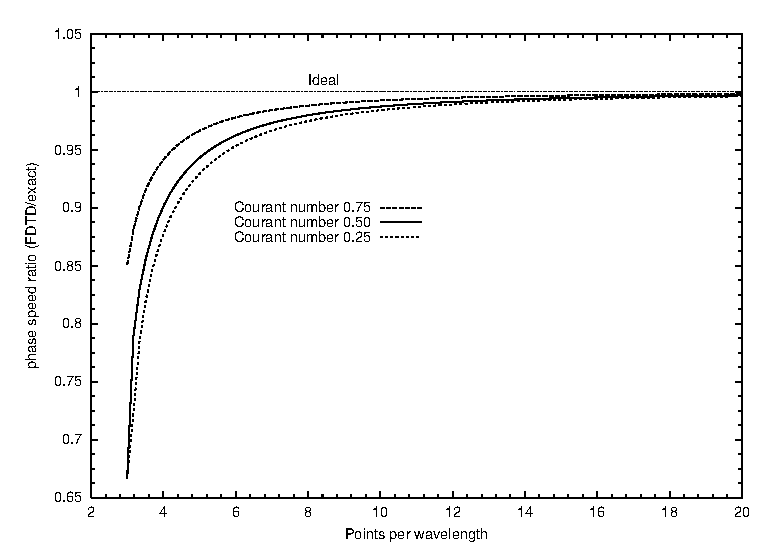
\epsfig{width=5.in,file=Code/Fdtd-dispersion/disp-error.eps}
  \end{center}
  \caption{Ratio of the FDTD and exact phase speeds
  ($\tilde{c}_p/c_p$) versus the discretization.  Propagation in free
  space is assumed.  Ideally the ratio would be unity for all
  discretizations.  Courant numbers of $1/4$, $1/2$, and $3/4$ are
  considered.}  \label{fig:dispError}
\end{figure}

Figure \ref{fig:dispDemo} shows snapshots of Ricker wavelets
propagating to the right that have been discretized at either $20$ or
$10$ points per wavelength at the most energetic frequency (i.e., the
parameter $N_P$ discussed in Sec.\ \ref{sec:ricker} is either $20$ or $10$).
The wavelets are propagating in grids that have a Courant number of
either $1$ or $0.5$.  In Figs.\ \ref{fig:dispDemo}(a) and (b) the
discretizations are $20$ and $10$, respectively, and the Courant
number is unity.  Since this corresponds to the magic time-step, the
wavelets propagate without distortion.  The discretizations in
Figs.\ \ref{fig:dispDemo}(c) and (d) are also $20$ and $10$,
respectively, but now the Courant number is $0.5$.  The snapshots in
(a) and (b) were taken after $100$ time-steps while the snapshots in
(c) and (d) were taken after $200$ time-steps (since the time step is
half as large in (c) and (d) as it is in (a) and (b), this ensures the
snapshots are depicting the field at the same time).  In
Fig.\ \ref{fig:dispDemo}(c) the distortion of the Ricker wavelet is
visible in that the function is no longer symmetric about the peak.
In Fig.\ \ref{fig:dispDemo}(d) the distortion caused by dispersion is
rather extreme and the function is no longer recognizable as a Ricker
wavelet.  The reason that Fig.\ \ref{fig:dispDemo}(d) is so much more
distorted than Fig.\ \ref{fig:dispDemo}(c) is that the spectral energy
lies at a coarser discretization.  The more coarsely a harmonic is
discretized, the more dispersion it will suffer---the higher
frequencies propagate more slowly than the lower frequencies.  This
causes the ringing that is evident on the trailing side of the pulse.

\begin{figure}
  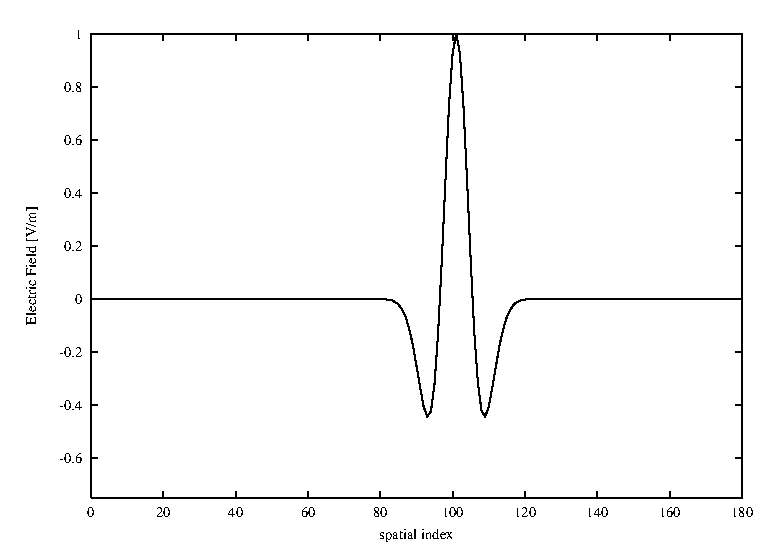
\epsfig{width=3.2in,file=Code/Fdtd-dispersion/disp-s1-ppw20.eps}
  \hspace{.1in}
  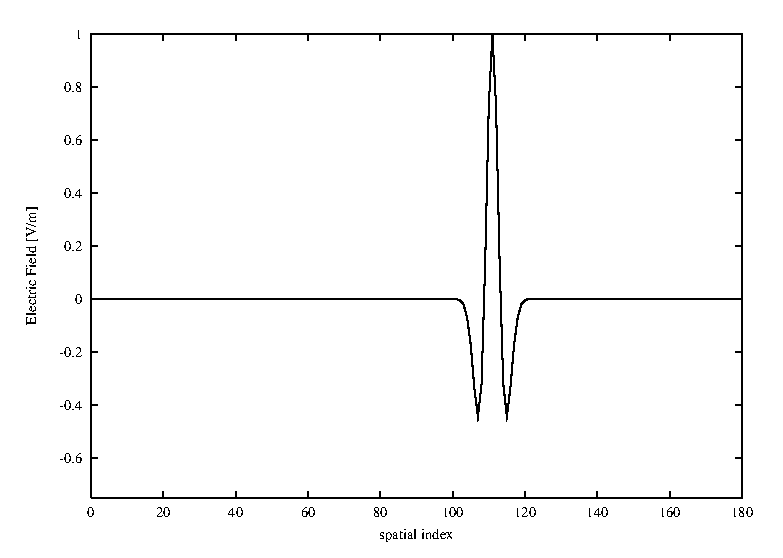
\epsfig{width=3.2in,file=Code/Fdtd-dispersion/disp-s1-ppw10.eps}\\
  \mbox{}\hspace{1.in}(a) $N_P=20$, $S_c=1$
         \hspace{1.95in}(b) $N_P=10$, $S_c=1$\\

  \vspace{.1in}
  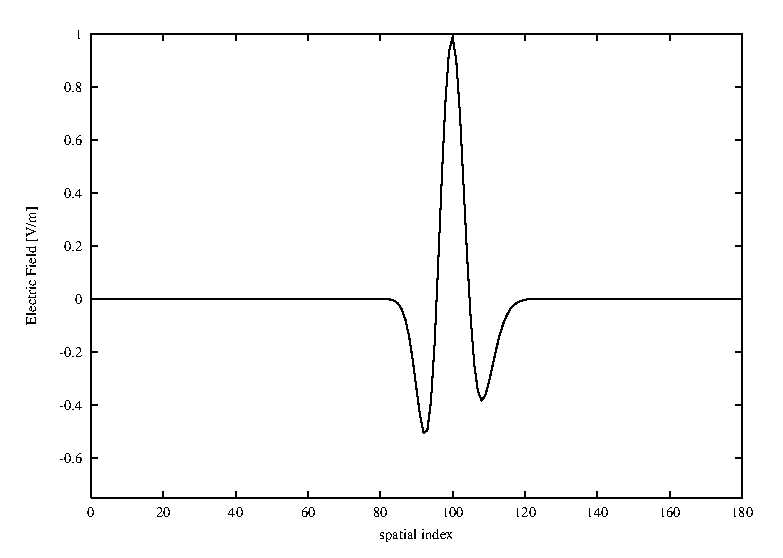
\epsfig{width=3.2in,file=Code/Fdtd-dispersion/disp-s0p5-ppw20.eps}
  \hspace{.1in}
  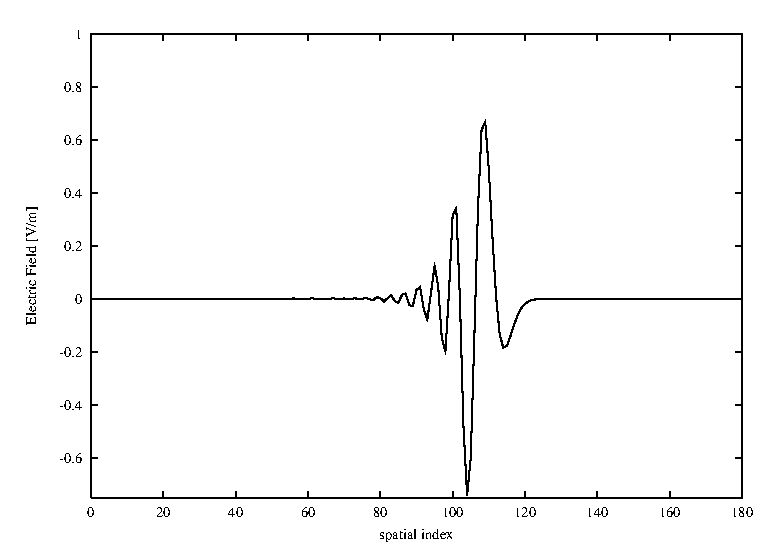
\epsfig{width=3.2in,file=Code/Fdtd-dispersion/disp-s0p5-ppw10.eps}\\
  \mbox{}\hspace{.95in}(c) $N_P=20$, $S_c=0.5$
         \hspace{1.95in}(d) $N_P=10$, $S_c=0.5$
  \caption{Snapshots of Ricker wavelets with different discretization
  propagating in grids with different Courant numbers.  (a) $20$
  points per wavelength at the most energetic frequency, i.e.,
  $N_P=20$, $S_c=1$, (b) $N_P=10$, $S_c=1$, (c) $N_P=20$, $S_c=0.5$,
  and (d) $N_P=10$, $S_c=0.5$.  The snapshots were taken after $100$
  time-steps for (a) and (b), and after $200$ time-steps for (c) and
  (d).}  \label{fig:dispDemo}
\end{figure}



\section{Numeric Impedance}

Let us return to \refeq{eq:dispAmperePart} which nominally gave the numeric
impedance and which is repeated below
\begin{equation}
  \frac{\hat{E}_0}{\hat{H}_0} = -\frac{K_x}{\epsilon\Omega}.
  \label{eq:impedance}
\end{equation}
The dispersion relation \refeq{eq:disp1DOmegaK} expressed $K_x$ in
terms of $\Omega$.  Plugging this into \refeq{eq:impedance} yields
\begin{equation}
  \frac{\hat{E}_0}{\hat{H}_0} =
     -\frac{\sqrt{\mu\epsilon}\Omega}{\epsilon\Omega} = 
     \sqrt{\frac{\mu}{\epsilon}} =
     \eta.
  \label{eq:impedanceI}
\end{equation}
Thus, despite the inherent approximations in the FDTD method, the
impedance in the grid is exactly the same as in the continuous world
(this also holds in higher dimensions).

\section{Analytic FDTD Reflection and Transmission
  Coefficients}

Section \ref{sec:measureTrans} discussed the way in which an FDTD
simulation could be used to measure the transmission coefficient
associated with a planar interface.  In this section, instead of using
a simulation to measure the transmission coefficient, an expression
will be derived that gives the transmission coefficient for the FDTD
grid.

Consider a one-dimensional FDTD simulation as shown in
Fig.\ \ref{fig:oneDHalfSpace}.  The permittivity changes abruptly at
the magnetic field which is assumed to coincide with the interface at
$x=0$.  The permeability is constant throughout the computational
domain.  

\begin{figure}
  \begin{center}
  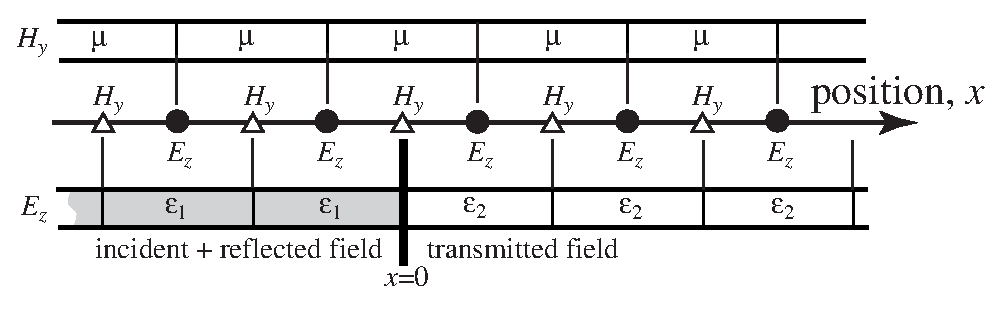
\epsfig{width=5.in,file=Figures/Fdtd-dispersion/dielectric-discontinuity.eps}
  \end{center} \caption{One-dimensional simulation where the
  permittivity changes abruptly at $x=0$.  The interface between the
  two media coincides with a magnetic-field node.  The permeability is
  assumed to be constant throughout the computational domain.  The
  figure depicts the nodes and the material values associated with
  their updates.  The field to the left of the interface is the sum of
  the incident and reflected fields.  The transmitted field exists to
  the right of the boundary.}  \label{fig:oneDHalfSpace}
\end{figure}

Assume there is an incident unit-amplitude plane wave propagating in
the $+x$ direction.  Because of the change in permittivity, a
reflected field will exist to the left of the boundary which
propagates in the $-x$ direction.  Additionally, there will be a
transmitted field which propagates to the right of the boundary.  The
incident, reflected, and transmitted electrics fields are given by
\begin{eqnarray}
   \Eifdtdq &=& \Eifdtd e^{j\omega q\Delt} =
                e^{-j\tbeta_1 m\Delx}e^{j\omega q\Delt},
     \label{eq:eInc} \\
   \Erfdtdq &=& \Erfdtd e^{j\omega q\Delt} =
                \Gfdtd e^{j\tbeta_1 m\Delx}e^{j\omega q\Delt}, \\
   \Etfdtdq &=& \Etfdtd e^{j\omega q\Delt} =
                \Tfdtd e^{-j\tbeta_2 m\Delx}e^{j\omega q\Delt}
     \label{eq:eTrans}
\end{eqnarray}
where $\Gfdtd$ and $\Tfdtd$ are the FDTD reflection and transmission
coefficients, respectively.  Note that all fields will have the
common temporal phase factor $\exp(j\omega q\Delt)$.  Therefore this
term will not be explicitly written (its existence is implicit in the
fact that we are doing harmonic analysis).

As shown in the previous section, the characteristic impedance in the
FDTD grid is exact.  Therefore the magnetic fields can be related to
the electric fields in the same manner as they are in the continuous
world, i.e.,
\begin{eqnarray}
   \Hifdtd &=& -\frac{1}{\eta_1}e^{-j\tbeta_1 m\Delx},
     \label{eq:hInc}\\
   \Hrfdtd &=& \frac{\Gfdtd }{\eta_1}e^{j\tbeta_1 m\Delx}, \\
   \Htfdtd &=& -\frac{\Tfdtd}{\eta_2} e^{-j\tbeta_2 m\Delx}.
     \label{eq:hTrans}
\end{eqnarray}

The incident and reflected waves exist to the left of the interface
and the transmitted field exists to the right of the interface.  The
magnetic field at the interface, i.e., the node at $x=0$ is, in a
sense, common to both the left and the right half-spaces.  The field
at this node can be described equally well as the sum of the
incident and reflected waves or by the transmitted wave.  This node
enforces the continuity of the magnetic field across the boundary.
Hence, just as in the continuous world, the fields are governed by the
equation
\begin{equation}
  -\frac{1}{\eta_1} + \frac{\Gfdtd}{\eta_1} = -\frac{\Tfdtd}{\eta_2}.
  \label{eq:magContinuity}
\end{equation}

In the continuous world enforcing the continuity of the tangential
electric and magnetic fields at a boundary yields two equations.
These two equations can be used to solve for the reflection and
transmission coefficients as was shown in Sec.\ \ref{sec:contTrans}.
In FDTD, however, there are no electric field nodes that coincide with
the interface (at least not with this geometry).  Therefore continuity
of the electric fields cannot be enforced directly nor is there a
readily available second equation with which to solve for the
reflection and transmission coefficients.

The necessary second equation is obtained by considering the update
equation for the magnetic field at the interface.  This node depends
on the electric field to either side of the interface and hence ties
the two half-spaces together.  Specifically, the harmonic form of
Faraday's law which governs the magnetic-field node at the interface
can be used to write the following
\begin{eqnarray}
  \left.\mu s_x^{1/2}\tpartial_t\fdtd{\hat{H}_y}{m}{q}\right|_{x=0} &=&
  \left.s_x^{1/2}\tpartial_x\fdtd{\hat{E}_z}{m}{}\right|_{x=0},
  \\
  \left.\mu j\Omega\fdtd{\hat{H}_y}{m}{}\right|_{x=0} &=&
  \left.\frac{1}{\Delx}\left(s_x^{1/2} - s_x^{-1/2}\right)
     \fdtd{\hat{E}_z}{m}{q}\right|_{x=0},
  \\
  \left.j\Omega \fdtd{\hat{H}_y}{m}{}\right|_{x=0} &=&
  \frac{1}{\mu\Delx}
     \left(\Tfdtd e^{-j\tbeta_2\Delx/2} - 
           \left[e^{j\tbeta_1\Delx/2} + \Gfdtd e^{-j\tbeta_1\Delx/2}\right]\right).
  \label{eq:interfaceEqII}
\end{eqnarray}
In the last form of the equation, we have used the fact that the
transmitted field is present when space is shifted a half spatial-step
in the $+x$ direction relative to the boundary.  Conversely the field
is the sum of the incident and reflected waves when space is shifted a
half spatial-step in the $-x$ direction relative to the boundary.

Equation \refeq{eq:interfaceEqII} provides the second equation which,
when coupled to \refeq{eq:magContinuity}, can be used to solve for the
transmission and reflection coefficients.  However, what is
$\left.\fdtd{\hat{H}_y}{m}{}\right|_{x=0}$?  Since this node is on the
interface, the expression for either the transmitted field or the sum
of the incident and reflected field can be used.  Using the
transmitted field (evaluated at $m=0$), the equation becomes
\begin{equation}
  j\Omega \left(-\frac{\Tfdtd}{\eta_2}\right) =
  \frac{1}{\mu\Delx}
     \left(\Tfdtd e^{-j\tbeta_2\Delx/2} - 
           \left[e^{j\tbeta_1\Delx/2} + \Gfdtd e^{-j\tbeta_1\Delx/2}\right]\right).
  \label{eq:usedTrans}
\end{equation}
Regrouping terms yields
\begin{equation}
  e^{j\tbeta_1\Delx/2} + \Gfdtd e^{-j\tbeta_1\Delx/2} =
  \left(e^{-j\tbeta_2\Delx/2} + j\frac{\Omega\mu\Delx}{\eta_2}\right) \Tfdtd.
  \label{eq:magContinuityI}
\end{equation}
After multiplying through by $-\eta_1\exp(-j\tbeta_1\Delx/2)$,
\refeq{eq:magContinuity} becomes
\begin{equation}
  e^{-j\tbeta_1\Delx/2} - \Gfdtd e^{-j\tbeta_1\Delx/2} =
  \frac{\eta_1}{\eta_2} e^{-j\tbeta_1\Delx/2} \Tfdtd.
  \label{eq:magContinuityII}
\end{equation}
Adding the left- and right-hand sides of \refeq{eq:magContinuityI} and
\refeq{eq:magContinuityII} yields an expression that does not depend
on the reflection coefficient.  Multiplying this expression through by
$\eta_2$ yields
\begin{equation}
  \eta_2\left(e^{j\tbeta_1\Delx/2} + e^{-j\tbeta_1\Delx/2}\right) =
  \left(\eta_1 e^{-j\tbeta_1\Delx} + \eta_2 e^{-j\tbeta_2\Delx/2} +
  j\Omega\mu\Delx\right) \Tfdtd.
  \label{eq:solvingForTrans}
\end{equation}
Let us consider the third term in parentheses on the right-hand side.
Recall from \refeq{eq:disp1DOmegaK} that $\Omega =
K_x/\sqrt{\mu\epsilon}$.  Taking the material and propagation
constants that pertain in the second medium,\footnote{As will be more
  obvious at the end of this derivation, we could instead select the
  material properties that pertain in the first medium and still obtain
  the same final result.} we can write
\begin{eqnarray}
  j\Omega\mu\Delx &=& 
    j\frac{K_{x2}}{\sqrt{\mu\epsilon_2}}\mu\Delx,
   \label{eq:transConversionI}
  \\
  &=&
   j\sqrt{\frac{\mu}{\epsilon_2}}\frac{2}{\Delx}
      \sin\left(\frac{\tbeta_2\Delx}{2}\right)\Delx,
   \label{eq:transConversionII}
  \\
  &=&
   j \eta_2 2
      \left(\frac{e^{j\tbeta_2\Delx/2} - e^{-j\tbeta_2\Delx/2}}{j2}\right),
 \\
  &=&
   \eta_2 \left(e^{j\tbeta_2\Delx/2} - e^{-j\tbeta_2\Delx/2}\right),
   \label{eq:transConversionIV}
\end{eqnarray}
where \refeq{eq:KxDefinition} was used to go from
\refeq{eq:transConversionI} to \refeq{eq:transConversionII}.  Plugging
this final form into \refeq{eq:solvingForTrans}, employing Euler's
formula, and solving for the transmission coefficient yields
\begin{equation}
  \Tfdtd = \frac{2 \eta_2 \cos\!\left(\frac{\tbeta_1\Delx}{2}\right)}
             {\eta_1 e^{-j\tbeta_1\Delx/2} + \eta_2 e^{j\tbeta_2\Delx/2}}.
  \label{eq:fdtdTransCoefMess}
\end{equation}
This can be compared to the exact transmission coefficient which is
given in \refeq{eq:transCoefSpectral}.  At first it may appear that
these are quite dissimilar.  However, if the discretization is
sufficiently small, the cosine and complex exponentials are close to
unity (and become one as the discretization goes to zero).  Hence the
FDTD reflection coefficient reduces to the exact reflection
coefficient as the discretization goes to zero.

The complex exponentials in \refeq{eq:fdtdTransCoefMess} make it
appear that the FDTD transmission coefficient is complex.  This would
impart a phase shift to the transmitted field that is not present in
the continuous world.  However, this is not the
case---\refeq{eq:fdtdTransCoefMess} can be simplified further.  The
one-dimensional dispersion relation \refeq{eq:disp1D} dictates that
\begin{equation}
  \sin\!\left(\frac{\tbeta\Delx}{2}\right) = 
  \frac{\sqrt{\epsilon\mu}\Delx}{\Delt}
  \sin\!\left(\frac{\omega\Delt}{2}\right).
  \label{eq:dispersionConversion}
\end{equation}
Now consider the denominator of \refeq{eq:fdtdTransCoefMess}
\begin{eqnarray}
  \lefteqn{\eta_1 e^{-j\tbeta_1\Delx/2} + \eta_2 e^{j\tbeta_2\Delx/2}} &&
  \nonumber
 \\
  &=&
    \eta_1\left(\cos\!\left(\frac{\tbeta_1\Delx}{2}\right)
               -j\sin\!\left(\frac{\tbeta_1\Delx}{2}\right)\right) + 
    \eta_2\left(\cos\!\left(\frac{\tbeta_2\Delx}{2}\right)
               +j\sin\!\left(\frac{\tbeta_2\Delx}{2}\right)\right)
\end{eqnarray}
Using \refeq{eq:dispersionConversion} to convert the sine terms and
employing the definition of impedance, the denominator can be written
\begin{eqnarray}
   \lefteqn{
    \eta_1\cos\!\left(\frac{\tbeta_1\Delx}{2}\right) + 
    \eta_2\cos\!\left(\frac{\tbeta_2\Delx}{2}\right)} &&
 \nonumber \\
  && \quad - j\sqrt{\frac{\mu}{\epsilon_1}}
              \frac{\sqrt{\epsilon_1\mu}\Delx}{\Delt}
                    \sin\!\left(\frac{\omega\Delt}{2}\right)
           + j\sqrt{\frac{\mu}{\epsilon_2}}
              \frac{\sqrt{\epsilon_2\mu}\Delx}{\Delt}
                    \sin\!\left(\frac{\omega\Delt}{2}\right).
\end{eqnarray}
Upon canceling the $\epsilon$'s, the imaginary parts cancel and hence
the denominator is purely real.  Therefore another expression for
the FDTD transmission coefficient is
\begin{equation}
  \Tfdtd = \frac{2 \eta_2 \cos\!\left(\frac{\tbeta_1\Delx}{2}\right)}
             {\eta_2 \cos\!\left(\frac{\tbeta_2\Delx}{2}\right)
            + \eta_1 \cos\!\left(\frac{\tbeta_1\Delx}{2}\right)}.
  \label{eq:fdtdTransCoef}
\end{equation}
Combining this with \refeq{eq:magContinuity} yields the reflection
coefficient
\begin{equation}
  \Gfdtd = \frac{\eta_2 \cos\!\left(\frac{\tbeta_2\Delx}{2}\right)
            - \eta_1 \cos\!\left(\frac{\tbeta_1\Delx}{2}\right)}
             {\eta_2 \cos\!\left(\frac{\tbeta_2\Delx}{2}\right)
            + \eta_1 \cos\!\left(\frac{\tbeta_1\Delx}{2}\right)}.
  \label{eq:fdtdRefCoef}
\end{equation}
Because the permeability is assumed to be constant throughout the
computational domain, the reflection and transmission coefficients can
be written as
\begin{eqnarray}
  \Tfdtd &=& \frac{2 \sqrt{\epsilon_1} \cos\!\left(\frac{\tbeta_1\Delx}{2}\right)}
             {\sqrt{\epsilon_1} \cos\!\left(\frac{\tbeta_2\Delx}{2}\right)
            + \sqrt{\epsilon_2} \cos\!\left(\frac{\tbeta_1\Delx}{2}\right)},
  \label{eq:fdtdTransCoefI}
  \\
  \Gfdtd &=& \frac{\sqrt{\epsilon_1} \cos\!\left(\frac{\tbeta_2\Delx}{2}\right)
            - \sqrt{\epsilon_2} \cos\!\left(\frac{\tbeta_1\Delx}{2}\right)}
             {\sqrt{\epsilon_1} \cos\!\left(\frac{\tbeta_2\Delx}{2}\right)
            + \sqrt{\epsilon_2} \cos\!\left(\frac{\tbeta_1\Delx}{2}\right)}.
  \label{eq:fdtdRefCoefI}
\end{eqnarray}

Figure \ref{fig:refCoefOneFour} shows a plot of the FDTD reflection
coefficient versus the points per wavelength (in free space) when a
wave is incident from free space to a dielectric with a relative
permittivity of $4.0$.  For these materials the exact reflection
coefficient, which is independent of the discretization and is also
shown in the plot, is $\hat{\Gamma} = (1-2)/(1+2) = -1/3$.  When the
discretization is $10$ points per wavelength the FDTD reflection
coefficient is nearly $-0.42$ which corresponds to an error of
approximately $26$ percent.  This error is rather large, but one must
keep in mind that in the dielectric the discretization is only five
points per wavelength.  This coarse discretization affects the quality
of the results throughout the computational domain, not just in the
dielectric.  Thus, even though one may ultimately be interested in the
fields over only a portion of the computational domain, nevertheless,
one must assure that a proper level of discretization is maintained
throughout the grid.

\begin{figure}
  \begin{center}
  \epsfig{width=4.in,angle=-90,file=Figures/Fdtd-dispersion/mag-ref.eps}
  \end{center} \caption{Reflection coefficient versus discretization
  for a wave traveling from free space to a dielectric with a relative
  permittivity of $4.0$ (i.e., $\epsilon_{r1} = 1.0$ and
  $\epsilon_{r2} = 4.0$).  The discretization $N_\lambda$ shown on the
  horizontal axis is that which pertains to free space.  (These values
  should be halved to give the discretization pertaining to the
  dielectric.)}
  \label{fig:refCoefOneFour}
\end{figure}

\section{Reflection from a PEC}

A perfect electric conductor is realized by setting to zero electric
field nodes.  Let us assume that one wants to continue to define the
interface as shown in Fig.\ \ref{fig:oneDHalfSpace}, i.e., the
boundary is assumed to coincide with a magnetic-field node.  The new
scenario is shown in Fig.\ \ref{fig:dielectricPEC}.  The
electric-field node to the right of the interface is set to zero.  We
now seek to find the reflection coefficient for this case.  There is
no transmitted field so the transmission coefficient $\Tfdtd$ must be
zero.  That might lead one to think, given \refeq{eq:magContinuity},
that the reflection coefficient must be $-1$ as it is in the
continuous world for a PEC boundary.  However, that is not correct.
Implicit in \refeq{eq:magContinuity} is the assumption that the
magnetic field is continuous across the interface.  When a PEC is
present, this is no longer the case.  In the continuous world the
discontinuity in the magnetic field is accounted for by a surface
current.

\begin{figure}
  \begin{center}
  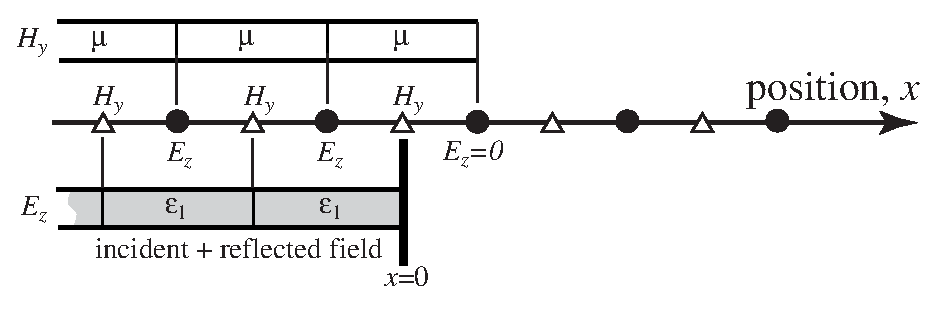
\epsfig{width=4.5in,file=Figures/Fdtd-dispersion/dielectric-pec.eps}
  \end{center}
  \caption{One-dimensional space with a perfect electric conductor
  realized by setting an electric field node to zero.  No fields
  propagate beyond the zeroed node.  The reference point $x=0$ is
  still assumed to coincide with a magnetic-field node.}
  \label{fig:dielectricPEC}
\end{figure}


When a PEC is present there is only one unknown, the reflection
coefficient can be obtained from a single equation since the
transmission coefficient is known {\em a priori}.  This equation is
provided, as before, by the update equation of the magnetic-field node
at the interface.  To this end, \refeq{eq:interfaceEqII} is used with
the transmission coefficient set to zero.  Also, instead of using the
transmitted form of the magnetic field at the interface as was done to
obtain \refeq{eq:usedTrans}, the sum of the incident and reflected
fields is used to obtain:
\begin{equation}
  j\Omega \left(-\frac{1}{\eta_1}+\frac{\Gfdtd}{\eta_1}\right) =
  \frac{1}{\mu\Delx}
     \left(0 - 
           \left[e^{j\tbeta_1\Delx/2} + \Gfdtd e^{-j\tbeta_1\Delx/2}\right]\right).
\end{equation}
Solving for the reflection coefficient yields
\begin{equation}
  \Gfdtd_{\mbox{\scriptsize PEC}} = 
  \frac{j\Omega\mu\Delx - \eta_1 e^{j\tbeta_1\Delx/2}}
       {j\Omega\mu\Delx + \eta_1 e^{-j\tbeta_1\Delx/2}}.
\end{equation}
As was shown in
\refeq{eq:transConversionI}--\refeq{eq:transConversionIV}, the factor
$j\Omega\mu\Delx$ can be expressed in terms of the impedance and a
difference of complex exponentials.  Employing such a conversion
allows the reflection coefficient to be written as
\begin{equation}
  \Gfdtd_{\mbox{\scriptsize PEC}} = -e^{-j\tbeta_1\Delx}.
  \label{eq:fdtdRefPEC}
\end{equation}
Note that the magnitude of the reflection coefficient is unity so that
the entire incident field, regardless of the frequency, is reflected from
the interface.

It appears that the FDTD reflection coefficient for a PEC is
introducing a shift that is not present in the continuous world.
However, this is being a bit unfair to the FDTD method.  The location
of the PEC boundary really corresponds to the electric-field node
that was set to zero.  Thus, one should really think of the PEC
boundary existing at $x=\Delx/2$.

In the continuous world, let us consider a scenario where the origin
is located a distance $\Delx/2$ in front of a PEC boundary.  In that
case the incident and reflected fields must sum to zero at
$x=\Delx/2$, i.e.,
\begin{eqnarray}
  \left.E^{\mbox{\scriptsize inc}}(x) + E^{\mbox{\scriptsize ref}}(x)
  \right|_{x=\Delx/2} &=& 0,\\
  e^{-j\beta_1\Delx/2} + \hat{\Gamma} e^{j\beta_1\Delx/2}  &=& 0.
\end{eqnarray}
Thus, in the continuous world the reflection coefficient is
\begin{equation}
 \hat{\Gamma} = -e^{-j\beta_1\Delx}.
 \label{eq:refContinuousPEC}
\end{equation}
When first comparing \refeq{eq:fdtdRefPEC}
and \refeq{eq:refContinuousPEC} it may appear that in this case the
FDTD reflection coefficient is exact.  However the two differ owing to
the fact that phase constants $\beta_1$ and $\tbeta_1$ are different
in the two domains.

\section{Interface Aligned with an Electric-Field Node}

There are situations which necessitate that a discontinuity in
permittivity be modeled as coinciding with an electric field node.
The permittivity that should be used to either side of the interface
is unambiguous but the permittivity of the node at the interface is
open to question since it is neither in one half-space nor the other.
This scenario was mentioned in Sec.\ \ref{sec:gridInhomogeneities}
where it was suggested that the average permittivity be used for the
node at the interface.  In this section we wish to provide a more
rigorous analysis to justify this permittivity.  For now, let the
permittivity of the node at the interface be $\epsilon_a$ as depicted
in Fig.\ \ref{fig:averageGeom}.  The goal now is to find the reflection or
transmission coefficients for this geometry and find the value of
$\epsilon_a$ which yields the best agreement with the continuous-world
values.

\begin{figure}
  \begin{center}
  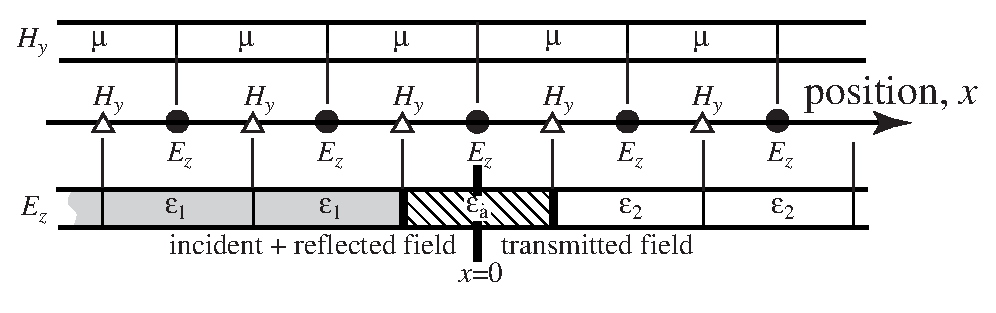
\epsfig{width=4.5in,file=Figures/Fdtd-dispersion/half-space-layer.eps}
  \end{center}
  \caption{One-dimensional space with a discontinuity in
  permittivity.  The interface in the continuous world corresponds to
  an electric-field node in the FDTD grid.  The permittivity to the
  left of the interface is $\epsilon_1$ and is $\epsilon_2$ to the
  right.  These values are dictated by those in the continuous world.
  The permittivity of the node at the interface is $\epsilon_a$.}
  \label{fig:averageGeom}
\end{figure}

Although the origin $x=0$ has shifted from that which was assumed in
the previous section, the incident, reflected, and transmitted fields
are still assumed to be given by \refeq{eq:eInc}--\refeq{eq:eTrans} and 
\refeq{eq:hInc}--\refeq{eq:hTrans}.  The electric-field node at the
interface is a member of both half-spaces, i.e., the field is the same
whether considered to be the sum of the incident and reflected field
or simply to be the transmitted field.  This yields a boundary
condition of
\begin{equation}
  1 + \Gfdtd = \Tfdtd.
  \label{eq:elecContinuity}
\end{equation}

Another equation relating the transmission and reflection coefficients
is obtained via the update equation for the electric-field node at the
interface.  Ampere's law evaluated at the interface is
\begin{equation}
  j\epsilon_a\Omega \Tfdtd = \frac{1}{\Delx}
  \left(-\frac{\Tfdtd}{\eta_2} e^{-j\tbeta_2\Delx/2} -
  \left[-\frac{1}{\eta_1} e^{j\tbeta_1\Delx/2} +
         \frac{\Gfdtd}{\eta_1} e^{-j\tbeta_1\Delx/2}\right]
  \right).
\end{equation}
Using \refeq{eq:elecContinuity} $\Tfdtd$ can be replaced with
$1+\Gfdtd$.  Then solving for $\Gfdtd$ yields
\begin{equation}
  \Gfdtd = \frac{\eta_2 e^{j\tbeta_1\Delx/2} - 
                 \eta_1 e^{-j\tbeta_2\Delx/2} - 
                 j\eta_1\eta_2\epsilon_a\Omega\Delx}
                {\eta_2 e^{-j\tbeta_1\Delx/2} +
                 \eta_1 e^{-j\tbeta_2\Delx/2} + 
                 j\eta_1\eta_2\epsilon_a\Omega\Delx}.
  \label{eq:gammaAverage}
\end{equation}
The term $\Omega\Delx$ can be written as
\begin{eqnarray}
  \Omega\Delx &=& \frac{2}{\Delt}
      \sin\!\left(\frac{\omega\Delt}{2}\right)\Delx, \\
  &=& 2c\frac{\Delx}{c\Delt}
      \sin\!\left(\frac{\omega\Delt}{2}\right), \\
  &=& 2c\frac{1}{S_c}
      \sin\!\left(\frac{2\pi c}{\ppw\Delx}\frac{\Delt}{2}\right), \\
  &=& 2c\frac{1}{S_c}
      \sin\!\left(\frac{\pi}{\ppw} S_c\right).
\end{eqnarray}
The conversion of $\omega\Delt/2$ to $\pi S_c/\ppw$ was discussed in
connection with \refeq{eq:lossTerm}.  Using this last form of
$\Omega\Delx$, the third term in the numerator and denominator of
\refeq{eq:gammaAverage} can be written
\begin{eqnarray}
  j\eta_1\eta_2\epsilon_a\Omega\Delx &=&
  j\sqrt{\frac{\mu}{\epsilon_0\epsilon_{r1}}}
   \sqrt{\frac{\mu}{\epsilon_0\epsilon_{r2}}}
  2c\epsilon_0\epsilon_{ra}\frac{1}{S_c}
      \sin\!\left(\frac{\pi}{\ppw} S_c\right), \\
  &=&
  j\frac{\epsilon_{ra}}{\sqrt{\epsilon_{r1}\epsilon_{r2}}}
   \frac{\mu}{\epsilon_0}
  2c\epsilon_0\frac{1}{S_c}
      \sin\!\left(\frac{\pi}{\ppw} S_c\right), \\
  &=&
  j\frac{\epsilon_{ra}}{\sqrt{\epsilon_{r1}\epsilon_{r2}}}
  2\mu c \frac{1}{S_c}
      \sin\!\left(\frac{\pi}{\ppw} S_c\right),
  \label{eq:interfaceTerm}
\end{eqnarray}
where $\epsilon_{ra}$ is the relative permittivity of the node at the
interface.

Assume that the permeability throughout the computational domain is
the permeability of free space so that $\mu c$ in
\refeq{eq:interfaceTerm} can be written $\mu_0
c=\mu_0/\sqrt{\mu_0\epsilon_0} = \sqrt{\mu_0/\epsilon_0} = \eta_0$.
The reflection coefficient \refeq{eq:gammaAverage} can now be written
as
\begin{equation}
  \Gfdtd = \frac{\frac{1}{\sqrt{\epsilon_{r2}}}\eta_0 e^{j\tbeta_1\Delx/2} - 
                \frac{1}{\sqrt{\epsilon_{r1}}}\eta_0 e^{-j\tbeta_2\Delx/2} - 
                j\frac{\epsilon_{ra}}{\sqrt{\epsilon_{r1}\epsilon_{r2}}}
                \eta_0 \frac{2}{S_c}
                \sin\!\left(\frac{\pi}{\ppw} S_c\right)}
              {\frac{1}{\sqrt{\epsilon_{r2}}}\eta_0 e^{-j\tbeta_1\Delx/2} +
                \frac{1}{\sqrt{\epsilon_{r1}}}\eta_0 e^{-j\tbeta_2\Delx/2} + 
                j\frac{\epsilon_{ra}}{\sqrt{\epsilon_{r1}\epsilon_{r2}}}
                \eta_0 \frac{2}{S_c}
                \sin\!\left(\frac{\pi}{\ppw} S_c\right)}.
  \label{eq:gammaAverageI}
\end{equation}
Multiplying numerator and denominator by
$\sqrt{\epsilon_{r1}\epsilon_{r2}}/\eta_0$ yields
\begin{equation}
  \Gfdtd = \frac{\sqrt{\epsilon_{r1}} e^{j\tbeta_1\Delx/2} - 
                 \sqrt{\epsilon_{r2}} e^{-j\tbeta_2\Delx/2} - 
                j \epsilon_{ra} \frac{2}{S_c}
                \sin\!\left(\frac{\pi}{\ppw} S_c\right)}
              {\sqrt{\epsilon_{r1}} e^{-j\tbeta_1\Delx/2} +
               \sqrt{\epsilon_{r2}} e^{-j\tbeta_2\Delx/2} + 
                j\epsilon_{ra} \frac{2}{S_c}
                \sin\!\left(\frac{\pi}{\ppw} S_c\right)}.
  \label{eq:gammaAverageII}
\end{equation}
As is often the case, the expression for a quantity in the FDTD grid
bears little resemblance to that in the continuous world.  However, as
the discretization goes to zero (i.e., $\ppw$ goes to infinity),
\refeq{eq:gammaAverageII} does indeed reduce to the reflection
coefficient in the continuous world.

The first two terms in the numerator and denominator of
\refeq{eq:gammaAverageII} depend on the material constants to either
side of the interface while the third term depends on the permittivity
at the interface, the Courant number, and the number of points per
wavelength (in continuous-world free space).  We now seek the value of
$\epsilon_a$ (or the corresponding relative permittivity
$\epsilon_{ra}$) which minimizes the difference between the reflection
coefficient in the continuous world and the one in the FDTD world.  It
is important to note that in general the FDTD reflection coefficient
in this case is truly complex---there will be a phase shift imparted
that does not exist in the continuous world.

Before going further with the analysis, let us consider an example
with specific parameters and graphically solve for the optimum value
of $\epsilon_a$.  Let $\epsilon_{r1} = 1$, $\epsilon_{r2} = 4$, and
the discretization be 10 points per wavelength.  In this case the
reflection coefficient in the continuous world is $-1/3$ (independent
of frequency).  Figure \ref{fig:refCoefLayer} shows the FDTD
reflection coefficient in the complex plane for various values of
$\epsilon_{ra}$.  The continuous-world result, i.e., the exact result,
is a single point on the negative real axis.  As $\epsilon_{ra}$
varies a curve is obtained in the complex plane which is closest to
the exact value when $\epsilon_{ra}$ is $2.5$ which is the arithmetic
average of $1$ and $4$.  Thus the optimum value for the interface
permittivity is the average of the permittivities to either side.
However, these results are only for a specific discretization and for
one set of permittivities.  Is the average value the optimum one for
all permittivities and discretizations?

\begin{figure}
  \begin{center}
  \epsfig{width=4.5in,file=Figures/Fdtd-dispersion/reflec-re-im.eps}
  \end{center}
  \caption{Curve showing the FDTD reflection coefficient in the
    complex plane as a function of $\epsilon_{ra}$ as $\epsilon_{ra}$
    varies between the relative permittivity to the left of the
    interface ($\epsilon_{ra}=1$) and the relative permittivity to the
    right of the interface ($\epsilon_{ra}=4$).  The value of
    $\epsilon_{ra}$ which minimizes the difference between the FDTD
    reflection coefficient and the exact value of $-1/3$ is the
    average permittivity, i.e., $\epsilon_{ra}=2.5$. }
  \label{fig:refCoefLayer}
\end{figure}

To answer this question, let us return to \refeq{eq:gammaAverage} and
separate the numerator and denominator into real and imaginary parts.
The result is
\begin{equation}
  \Gfdtd = \frac
   {\eta_2\cos(\kappa_1) - \eta_1\cos(\kappa_2) +
     j\left[\eta_2\sin(\kappa_1) + \eta_1\sin(\kappa_2)
      -\eta_1\eta_2\epsilon_a\Omega\Delx\right]}
   {\eta_2\cos(\kappa_1) + \eta_1\cos(\kappa_2) -
     j\left[\eta_2\sin(\kappa_1) + \eta_1\sin(\kappa_2)
      -\eta_1\eta_2\epsilon_a\Omega\Delx\right]}
\end{equation}
where
\begin{eqnarray}
  \kappa_1 &=& \tbeta_1\Delx/2, \\
  \kappa_2 &=& \tbeta_2\Delx/2.
\end{eqnarray}
The continuous-world reflection coefficient is purely real and thus
any imaginary part is an error.  Furthermore, the imaginary part goes
to zero as the discretization goes to zero.  Let us consider just this
imaginary part of the numerator and denominator.  The $\sin(\kappa)$
terms can be related to the $K$ terms which have been used
previously---one merely had to multiply (and divide) by $2/\Delx$.
Thus the imaginary part can be written
\begin{equation}
  \eta_2\frac{2}{\Delx}\sin(\kappa_1)\frac{\Delx}{2} +
  \eta_1\frac{2}{\Delx}\sin(\kappa_2)\frac{\Delx}{2} -
  \eta_1\eta_2\epsilon_a\Omega\Delx
   =
  \eta_1\eta_2\frac{\Delx}{2}\left(\frac{1}{\eta_1}K_1 + 
                    \frac{1}{\eta_2}K_2 -
                    2\epsilon_a\Omega\right).
\end{equation}
From the dispersion relation \ref{eq:fdtdDispersionOneD} we know that
$K_1=\sqrt{\mu\epsilon_1}\Omega$ and $K_2=\sqrt{\mu\epsilon_2}\Omega$.
This allows the imaginary part of the numerator and denominator of the
reflection coefficient to be written
\begin{equation}
  \eta_1\eta_2\frac{\Delx}{2}\Omega
  \left(\epsilon_1 + \epsilon_2 - 2 \epsilon_a\right).
\end{equation}
Setting $\epsilon_a$ equal to $(\epsilon_1+\epsilon_2)/2$ will yield
zero for this imaginary term.  Hence the average permittivity is the
optimum value for all permittivities and discretizations!  Using the
average permittivity yields reflection and transmission coefficients of 
\begin{eqnarray}
  \Gfdtd &=& 
  \frac
   {\eta_2\cos(\kappa_1) - \eta_1\cos(\kappa_2)}
   {\eta_2\cos(\kappa_1) + \eta_1\cos(\kappa_2)}, \\
  \Tfdtd &=& 
  \frac
   {2\eta_2\cos(\kappa_1)}
   {\eta_2\cos(\kappa_1) + \eta_1\cos(\kappa_2)}.
\end{eqnarray}
Note that these equations appear almost identical to those
which pertained to the case of an abrupt interface (i.e., when no
averaging is done and the resulting reflection and transmission
coefficients are \refeq{eq:fdtdRefCoef} and
\refeq{eq:fdtdTransCoef}).  However, these equations differ in the
arguments of the cosine terms and, in fact, it can be shown that the
abrupt boundary is slightly more accurate than the one which is
implemented with the average permittivity at the interface.
Nevertheless, when the situation calls for the interface to coincide
with a tangential electric field, the average permittivity is the
optimum one to use.

